\documentclass[12pt,a4paper]{report}
\usepackage[utf8]{inputenc}
\usepackage[russian]{babel}
\usepackage[OT1]{fontenc}
\usepackage{amsmath}
\usepackage{amsfonts}
\usepackage{amssymb}
\usepackage{graphicx}
\usepackage{cmap}					% поиск в PDF
\usepackage{mathtext} 				% русские буквы в формулах
%\usepackage{tikz-uml}               % uml диаграммы

% TODOs
\usepackage[%
  colorinlistoftodos,
  shadow
]{todonotes}

% Генератор текста
\usepackage{blindtext}

%------------------------------------------------------------------------------

% Подсветка синтаксиса
\usepackage{color}
\usepackage{xcolor}
\usepackage{listings}
 
 % Цвета для кода
\definecolor{string}{HTML}{B40000} % цвет строк в коде
\definecolor{comment}{HTML}{008000} % цвет комментариев в коде
\definecolor{keyword}{HTML}{1A00FF} % цвет ключевых слов в коде
\definecolor{morecomment}{HTML}{8000FF} % цвет include и других элементов в коде
\definecolor{captiontext}{HTML}{FFFFFF} % цвет текста заголовка в коде
\definecolor{captionbk}{HTML}{999999} % цвет фона заголовка в коде
\definecolor{bk}{HTML}{FFFFFF} % цвет фона в коде
\definecolor{frame}{HTML}{999999} % цвет рамки в коде
\definecolor{brackets}{HTML}{B40000} % цвет скобок в коде
\DeclareGraphicsExtensions{.pdf,.png,.jpg}

 % Настройки отображения кода
\lstset{
language=C, % Язык кода по умолчанию
morekeywords={*,...}, % если хотите добавить ключевые слова, то добавляйте
 % Цвета
keywordstyle=\color{keyword}\ttfamily\bfseries,
stringstyle=\color{string}\ttfamily,
commentstyle=\color{comment}\ttfamily\itshape,
morecomment=[l][\color{morecomment}]{\#}, 
 % Настройки отображения     
breaklines=true, % Перенос длинных строк
basicstyle=\ttfamily\footnotesize, % Шрифт для отображения кода
backgroundcolor=\color{bk}, % Цвет фона кода
%frame=lrb,xleftmargin=\fboxsep,xrightmargin=-\fboxsep, % Рамка, подогнанная к заголовку
frame=tblr
rulecolor=\color{frame}, % Цвет рамки
tabsize=3, % Размер табуляции в пробелах
 % Настройка отображения номеров строк. Если не нужно, то удалите весь блок
numbers=left, % Слева отображаются номера строк
stepnumber=1, % Каждую строку нумеровать
numbersep=5pt, % Отступ от кода 
numberstyle=\small\color{black}, % Стиль написания номеров строк
 % Для отображения русского языка
extendedchars=true,
literate={Ö}{{\"O}}1
  {Ä}{{\"A}}1
  {Ü}{{\"U}}1
  {ß}{{\ss}}1
  {ü}{{\"u}}1
  {ä}{{\"a}}1
  {ö}{{\"o}}1
  {~}{{\textasciitilde}}1
  {а}{{\selectfont\char224}}1
  {б}{{\selectfont\char225}}1
  {в}{{\selectfont\char226}}1
  {г}{{\selectfont\char227}}1
  {д}{{\selectfont\char228}}1
  {е}{{\selectfont\char229}}1
  {ё}{{\"e}}1
  {ж}{{\selectfont\char230}}1
  {з}{{\selectfont\char231}}1
  {и}{{\selectfont\char232}}1
  {й}{{\selectfont\char233}}1
  {к}{{\selectfont\char234}}1
  {л}{{\selectfont\char235}}1
  {м}{{\selectfont\char236}}1
  {н}{{\selectfont\char237}}1
  {о}{{\selectfont\char238}}1
  {п}{{\selectfont\char239}}1
  {р}{{\selectfont\char240}}1
  {с}{{\selectfont\char241}}1
  {т}{{\selectfont\char242}}1
  {у}{{\selectfont\char243}}1
  {ф}{{\selectfont\char244}}1
  {х}{{\selectfont\char245}}1
  {ц}{{\selectfont\char246}}1
  {ч}{{\selectfont\char247}}1
  {ш}{{\selectfont\char248}}1
  {щ}{{\selectfont\char249}}1
  {ъ}{{\selectfont\char250}}1
  {ы}{{\selectfont\char251}}1
  {ь}{{\selectfont\char252}}1
  {э}{{\selectfont\char253}}1
  {ю}{{\selectfont\char254}}1
  {я}{{\selectfont\char255}}1
  {А}{{\selectfont\char192}}1
  {Б}{{\selectfont\char193}}1
  {В}{{\selectfont\char194}}1
  {Г}{{\selectfont\char195}}1
  {Д}{{\selectfont\char196}}1
  {Е}{{\selectfont\char197}}1
  {Ё}{{\"E}}1
  {Ж}{{\selectfont\char198}}1
  {З}{{\selectfont\char199}}1
  {И}{{\selectfont\char200}}1
  {Й}{{\selectfont\char201}}1
  {К}{{\selectfont\char202}}1
  {Л}{{\selectfont\char203}}1
  {М}{{\selectfont\char204}}1
  {Н}{{\selectfont\char205}}1
  {О}{{\selectfont\char206}}1
  {П}{{\selectfont\char207}}1
  {Р}{{\selectfont\char208}}1
  {С}{{\selectfont\char209}}1
  {Т}{{\selectfont\char210}}1
  {У}{{\selectfont\char211}}1
  {Ф}{{\selectfont\char212}}1
  {Х}{{\selectfont\char213}}1
  {Ц}{{\selectfont\char214}}1
  {Ч}{{\selectfont\char215}}1
  {Ш}{{\selectfont\char216}}1
  {Щ}{{\selectfont\char217}}1
  {Ъ}{{\selectfont\char218}}1
  {Ы}{{\selectfont\char219}}1
  {Ь}{{\selectfont\char220}}1
  {Э}{{\selectfont\char221}}1
  {Ю}{{\selectfont\char222}}1
  {Я}{{\selectfont\char223}}1
  {і}{{\selectfont\char105}}1
  {ї}{{\selectfont\char168}}1
  {є}{{\selectfont\char185}}1
  {ґ}{{\selectfont\char160}}1
  {І}{{\selectfont\char73}}1
  {Ї}{{\selectfont\char136}}1
  {Є}{{\selectfont\char153}}1
  {Ґ}{{\selectfont\char128}}1
  {\{}{{{\color{brackets}\{}}}1 % Цвет скобок {
  {\}}{{{\color{brackets}\}}}}1 % Цвет скобок }
}
 
 % Для настройки заголовка кода
\usepackage{caption}
\DeclareCaptionFont{white}{\color{сaptiontext}}
\DeclareCaptionFormat{listing}{\parbox{\linewidth}{\colorbox{сaptionbk}{\parbox{\linewidth}{#1#2#3}}\vskip-4pt}}
\captionsetup[lstlisting]{format=listing,labelfont=white,textfont=white}
\renewcommand{\lstlistingname}{Код} % Переименование Listings в нужное именование структуры


%------------------------------------------------------------------------------

\author{С.~А.~Климов}
\title{Сети ЭВМ и телекоммуникации}
\begin{document}
%\listoftodos
\maketitle
\chapter{Задание}
Разработать приложение-клиент и приложение сервер электронной почты.
\section{Функциональные требования}
%\todo[inline]{Начать можно с этого}
Серверное приложение должно реализовывать следующие функции:
\begin{enumerate}
\item Приём почтового сообщения от одного клиента для другого
\item Хранение электронной почты для клиентов
\item Посылка клиенту почтового сообщения по запросу с последующим
удалением сообщения
\item Посылка клиенту сведений о состоянии постового ящика
\item Обработка запроса на отключение клиента
\item Принудительное отключение клиента
\end{enumerate}
Клиентское приложение должно реализовывать следующие функции:
\begin{enumerate}
\item Передача электронного письма на сервер для другого клиента
\item Проверка состояния своего почтового ящика
\item Получение конкретного письма с сервера
\item Разрыв соединения
\item Обработка ситуации отключения клиента сервером
\end{enumerate}
\section{Нефункциональные требования}
Для сервера:
\begin{enumerate}
\item Прослушивание определенного порта
\item Поддержка одновременной работы нескольких почтовых клиентов
через механизм нитей
\item Обработка запросов на подключение по этому порту от клиентов
\end{enumerate}
Для клиента:
\begin{enumerate}
\item Установление соединения с сервером
\end{enumerate}
\section{Настройки приложений}
Разработанное клиентское приложение должно предоставлять пользова-
телю настройку IP-адреса или доменного имени удалённого сервера те-
стов и номера порта, используемого сервером. Разработанное серверное
приложение должно хранить вопросы и правильные ответы нескольких
тестов.
\section{Накладываемые ограничения}

Пакеты для обмена по протоколу TCP будут иметь размер 1024 байта. В пакетах под имя клиента выделяется до 20-ти символов, 1 символ команды, 3 разделяющих симовла, остальные 1000 символов выделяется под отправляемое сообщение. Этой длины достаточно для отправки писем средней длины.%Для установки корректной TCP сессии с удаленным хостом должно соблюдаться условие:
%\begin{math}
%MSS + TCP + IP \leqslant MTU.
%\end{math}


%Имя пользователя не должно превышать 20-ти символов для удобства ввода.
%Сообщение не дожно превышать 1000 символов для умеренной нагрузки сети.
Одновременное количесво подключенных к серверу клиентов как минимум до 5.

\chapter{Реализация для работы по протоколу TCP}
\section{Прикладной протокол}
\label{protocol_tcp}
\begin{tabular}{|c|c|}
\hline 
Первая команда ввода имя пользователя & username\# \\ 
\hline 
Команда написать kitty сщщбщение hello! & 1\#kitty\#hello!\# \\ 
\hline 
Команда прочитать входящие & 2\# \\
\hline 
Команда выхода & 3\# \\
\hline 
\end{tabular} 

\section{Архитектура приложения}
Взаимодействие сервера и клиента:
\begin{enumerate}
\item Сервер отправляет приветственное сообщение в котором клиенту предлагается ввести свой логин для идентификации его на сервере.
\item Клиент отправляет серверу свой логин.
\item Сервер отсылает клиенту список поддерживаемых команд(отослать письмо, прочитать входящие письма или выйти).
\item Клиент производит взаимодействие с сервером по средством ввода предложенных команд.
\item Клиент завершает работу с сервером.
\end{enumerate}
%Взаимодействие сервера и клиента начинается с отправки сервером приветственного сообщения в котором клиенту предлагается ввести свой логин для идентификации его на сервере. Затем, когда клиент отправит свой логин, сервер отсылает ему список поддерживаемых команд(отослать письмо, прочитать входящие письма или выйти). Далее клиент вводит нужные для него команды для взаимодействия с сервером. 
%Взаимодействие сервера и клиента начинается с отправки клиентом сообщение с его логином. Так сервер идентифицирует его в системе. Затем клиент посылает серверу разлчиные команды, он может отправить сообщение, прочитать свою почту и выйти.
\pagebreak
\flushleft
Sequence диаграмма, демонстрирующая возможное взаимодействие клиента и сервера:
\linebreak
\center \includegraphics[scale=0.8]{commun1.jpg}
\flushleft
%\begin{figure}[p]
 %   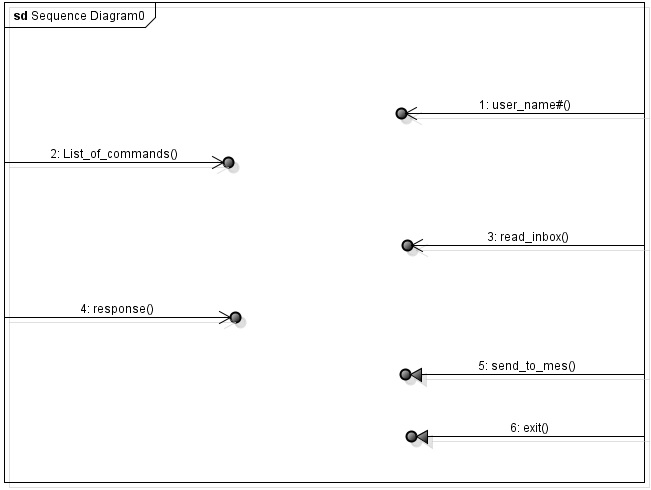
\includegraphics{TCP_comm.jpg}
%\end{figure}

Почта для каждого клиента хранится на сервере в виде xml файла, имя которого совпадает с именем пользователя.

XML-Schema структуры файлов со входящими сообщениями:
\lstinputlisting{xml_schema1.xsd}


\section{Тестирование}
\subsection{Описание тестового стенда и методики тестирования}
Тестирование проводилось на виртуальной машине Debian 4.7. Было запущено приложение сервера, затем - несколько приложений клента. Таким образом сервер и клиент работали на одном компьютере.
\subsection{Тестовый план и результаты тестирования}
%По шагам, с перечнем входных данных
\begin{enumerate}
\item На первом клиенте был осуществлен вход под логином "serg" и было отправлнео сообщение "hello!" клиенту "ali"
\item Был получен список входящих сообщений для пользователя "serg".
\item В другом терминале был запущен клиент с именем "ali"(терминал пользователя "serg" оставался активным).
\item Был получен список входящих сообщений, последним из них оказалось только что отправленное сообщение("hello!") пользователем "serg".
\item Было отправлено сообщение "nice to meet you!" пользователю "serg" и осуществлен выход.
\item На терминале пользователя "serg" были прочитаны сообщения, последним из них оказалось только что отправленное сообщение("nice to meet you!") пользователем "ali".
\item Был осуществлен выход пользователя "serg".
\end{enumerate}
%На первом клиенте был осуществлен вход под логином "serg", было отправлнео сообщение клиенту "ali". Был получен список входящих сообщений для пользователя "serg". В другом терминале был запущен клиент с именем "ali"(терминал пользователя "serg" оставался активным), далее был получен для него список входящих сообщений, последним из них оказалось только что отправленное сообщение пользователем "serg". Было отправлено сообщение пользователю "serg" и осуществлен выход. На терминале пользователя "serg" были прочитаны сообщения, последним из них оказалось только что отправленное сообщение пользователем "ali". Был осуществлен выход.
Ожидалось получить корректное взаимодействие сервера с клиентами, что и было получено: сервер корректно работает с несколькими клиентами.
При вводе некорректных команд клиентское приложение сообщает об этом пользователю и продолжает работу. Серверное приложение так же выводит на консоль некорректные команды от пользователя.
\linebreak
\linebreak
Тестирование работы сервера с большим количесвом клиентов:
\begin{enumerate}
\item Был запущен сервер.
\item Из различных терминалов было осуществлено подключение 5 клиентов.
\item Для каждого из клиентов была осуществлена отправка сообщения какому-либо пользователю.
\item Для каждого из клиентов был получен список писем.
\item Был осуществлен выход клиентами.
\end{enumerate}
Ожидалось получить корректное взаимодействие сервера с данным количеством клиентов, это и было получено: клиенты корректно отправляют сообщения друг другу и осуществляют просмотр входящих сообщений.
\chapter{Реализация для работы по протоколу UDP}
\section{Прикладной протокол}
Прикладной протокол понес небольшие изменения по сравнению с UDP. Однако для пользователя взаимодействие с сервером осалось аналогичным.
%Прикладной протокол остался таким же, как и в TCP, т.е. для пользователя взаимодействие совершенно аналогичо. Однако в самой реализации взаимодействие изменилось:


\section{Архитектура приложения}
Взаимодействие сервера и клиента:
\begin{enumerate}
\item Клиент отправляет серверу приветственное сообщение для начала взаимодействия.
\item Сервер отвечает ему сообщением в котором клиенту предлагается ввести свой логин для идентификации его на сервере.
\item Клиент отправляет серверу свой логин.
\item Сервер отсылает клиенту список поддерживаемых команд(отослать письмо, прочитать входящие письма или выйти).
\item Клиент производит взаимодействие с сервером по средством ввода предложенных команд.
\item Клиент завершает работу с сервером.
\end{enumerate}

Sequence диаграмма, демонстрирующая возможное взаимодействие клиента и сервера:
\linebreak
\center \includegraphics[scale=0.8]{commun_udp.jpg}
\flushleft

Изменение понес процесс отправки списка всех сообщений клиенту, если в TCP просто осущесвляется потоковая передача, то в UDP мы принимаем пакеты, пока не придет пакет определнного за ранее содержания, сигнализирующий о конце отправки писем.
\linebreak
\linebreak
Sequence диаграмма, демонстрирующая взаимодействие при получении клиентом списка сообщений от сервера:
\linebreak
\center \includegraphics[scale=0.8]{commun_read_udp.jpg}
\flushleft

Почта также хранится в xml файлах, как и в TCP. XML-Schema структуры файлов со входящими сообщениями аналогична.

%Взаимодействие сервера и клиента начинается с отправки клиентом приветственного сообщение, по этому сообщению сервер отсылает в ответ строку с предложением ввести свой логин.Клиент отправляет свой логин. Так сервер идентифицирует его в системе. Сервер отсылает строку с возможными командыми. Затем клиент посылает серверу разлчиные команды, он может отправить сообщение, прочитать свою почту и выйти.
%\linebreak
%\center 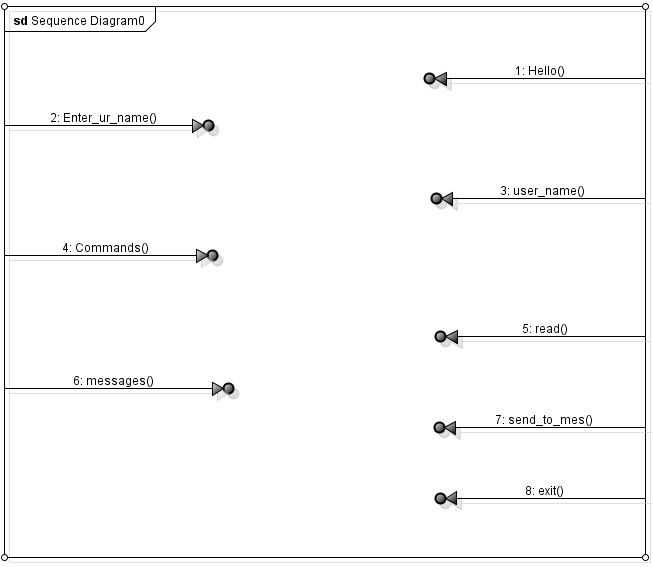
\includegraphics[scale=0.8]{UDP_comm.jpg}
%\flushleft

\section{Тестирование}
\subsection{Описание тестового стенда и методики тестирования}
Тестирование проводилось на виртуальной машине Debian 4.7. Было запущено приложение сервера, затем - несколько приложений клента. Таким образом сервер и клиент работали на одном компьютере.
\subsection{Тестовый план и результаты тестирования}
\begin{enumerate}
\item На первом клиенте был осуществлен вход под логином "serg" и было отправлнео сообщение "hello!" клиенту "ali"
\item Был получен список входящих сообщений для пользователя "serg".
\item В другом терминале был запущен клиент с именем "ali"(терминал пользователя "serg" оставался активным).
\item Был получен список входящих сообщений, последним из них оказалось только что отправленное сообщение("hello!") пользователем "serg".
\item Было отправлено сообщение "nice to meet you!" пользователю "serg" и осуществлен выход.
\item На терминале пользователя "serg" были прочитаны сообщения, последним из них оказалось только что отправленное сообщение("nice to meet you!") пользователем "ali".
\item Был осуществлен выход пользователя "serg".
\end{enumerate}
Ожидалось получить корректное взаимодействие сервера с клиентами, что и было получено: сервер корректно работает с несколькими клиентами.
При вводе некорректных команд клиентское приложение сообщает об этом пользователю и продолжает работу. Серверное приложение так же выводит на консоль некорректные команды от пользователя.
\linebreak
\linebreak
Тестирование работы сервера с большим количесвом клиентов:
\begin{enumerate}
\item Был запущен сервер.
\item Из различных терминалов было осуществлено подключение 5 клиентов.
\item Для каждого из клиентов была осуществлена отправка сообщения какому-либо пользователю.
\item Для каждого из клиентов был получен список писем.
\item Был осуществлен выход клиентами.
\end{enumerate}
Ожидалось получить корректное взаимодействие сервера с данным количеством клиентов, это и было получено: клиенты корректно отправляют сообщения друг другу и осуществляют просмотр входящих сообщений.
%По шагам, с перечнем входных данных
%На первом клиенте был осуществлен вход под логином "serg", было отправлнео сообщение клиенту "ali". Был получен список входящих сообщений для пользователя "serg". В другом терминале был запущен клиент с именем "ali"(терминал пользователя "serg" оставался активным), далее был получен для него список входящих сообщений, последним из них оказалось только что отправленное сообщение пользователем "serg". Было отправлено сообщение пользователю "serg" и осуществлен выход. На терминале пользователя "serg" были прочитаны сообщения, последним из них оказалось только что отправленное сообщение пользователем "ali". Был осуществлен выход.
%При вводе некорректных команд клиентское приложение сообщает об этом пользователю и продолжает работу. Серверное приложение так же выводит на консоль не корректные команды от пользователя.
\chapter{Выводы}
%Анализ выполненных заданий, сравнение удобства/эффективности/количества проблем при программировании TCP/UDP
\section{TCP}
%Когда взаимодействие осуществляется через TCP, обеспечивается надежная передача потока байтов как от приложения сервера к приложению клиента, так и в обратном направлении. Также использование TCP удобно, потому что осуществляется контроль длины сообщения, скорость обмена сообщениями и сетевой трафик средствами самого протокола TCP. 
Протокол ТСР является ориентированным на создание соединения, в нем производится так называемое "рукопожатие" для его установки. При установлении соединения становится возможной передача данных в обоих направлениях.
\linebreak
ТСР является надежным протоколом, т.к. он управляет подтверждением, повторной передачаей и тайм-аутом сообщений. Также ТСР осуществляет контроль порядка доставки сообщений, т.е. если сообщения доставляются не друг за другом, а в случайном порядке, то они внчале кешируются, а затем упорядочиваются и только потом передаются приложению.
Важной особенностью ТСР является то, что данные считываются как единый поток байтов, нет никаких границ для отдельных сообщений.
Очевидным достоинством ТСР является его надежность. Однако, при реализации приложния с его использованием можно столкнуться со следующими трудностями: организация работы сервера с несколькими клиентами. Для взаимодействия с несколькими клиентами серверу необходимо создавать новый сокет для каждого из них и передавать управление в отдельную нить, организуемую для обслуживания клиента.

\section{UDP}
Протокол UDP является более простым протоколом, нежели ТСР. Он не основан на установлении соединения, а просто и спользует механизм обмена дэйтаграммами для взаимодействия с клиентом.
\linebreak
Протокол UDP считается ненадежным, т.к. он не управляет подтверждением, повторной передачаей и тайм-аутом сообщений. Он не осуществляет контроль порядка передачи дэйтаграммм. Дэйтаграммы имеют определенные границы, т.е. они интерпретируются на приемной стороне однозначно, их целостность проверяется только после получения.
Важной особенностью UDP является его простота - нет механизма "рукопожатия", упорядочивания и отслеживания соединений.
Хотя UDP является болле простым, на разработчика ложатся дополнительные задачи при его использовании. Необходимо обеспечить контроль очередности доставки пакетов и повторную их отправку при потере пакета. При реализации взаимодействия с несколькими клиентами сервер, в отличии от ТСР, использует только один поток для их обслуживания. Это не дает возможности параллельной работы со всеми клиентами, применением мьютексов также не удалось решить данную проблему.
\linebreak
Как показало тестирование, реалиованные приложения как с использованим ТСР, так и UDP работают корректно.
%Когда взаимодействие осуществляется через UDP, не применяется модель взаимодействия клиента и сервера, использующая так называемые "неявные" рукопожатия. Из-за этого не осуществляется упорядочивание и контроль целостности данных средсвтами самого протокола, это приходится реализовывать вручную. Использование UDP накладывает на разработчка ряд дополнительных задач, такие как контроль целостности данных и их упорядочивание.
%\linebreak
%\linebreak
%При дальнейшей разработке сетевых приложений я бы использовал протокол TCP, т.к. он удобнее и легче в реализации.

\chapter{Приложения}
\section{Описание среды разработки}
%Версии ОС, компиляторов, утилит, и проч., которые использовались в процессе разработки
Linux Debian 7.6: Среда разработки - Eclipse.\linebreak
Windows 8.1: Среда разработки - Visual Studio 2013.
\section{Листинги}
\subsection{Сервер TCP. Основной файл программы main.c}
\lstinputlisting{./Server1/main.c}
%{/home/user/workspace/tcp_server/main.c}
\subsection{Сервер TCP. Файл сборки Makefile}
\lstinputlisting{./Server1/Makefile.make}
\subsection{Клиент TCP. Основной файл программы main.c}
\lstinputlisting{./Client1/main.c}
%{/home/user/workspace/tcp_server/main.c}
\subsection{Клиент TCP. Файл сборки Makefile}
\lstinputlisting{./Client1/Makefile.make}
\subsection{Сервер UDP. Основной файл программы main.c}
\lstinputlisting{./Server3/main.c}
\subsection{Сервер UDP. Файл сборки Makefile}
\lstinputlisting{./Server3/Makefile.make}
\subsection{Клиент UDP. Основной файл программы main.c}
\lstinputlisting{./Client3/main.c}
%{/home/user/workspace/tcp_server/main.c}
\subsection{Клиент UDP. Файл сборки Makefile}
\lstinputlisting{./Client3/Makefile.make}
%\todo[inline]{Не забыть вставить все исходники}
\end{document}